\section*{Лекція 13: Модулі та імпорт}
 
 \subsection{Імпорт модулів} 
\begin{frame}
\frametitle{Стандартні модулі Python}
\begin{figure}
  \begin{center}
    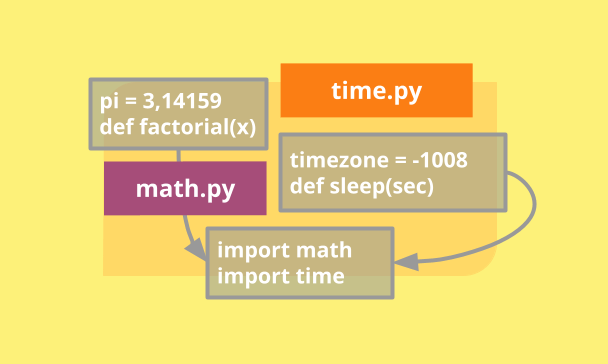
\includegraphics[width=0.4\textwidth,height=0.35\textheight]{pictures/import.png}
  \caption{Модулі Python}
\label{function}
  \end{center}
\end{figure}


Python має велику кількість стандартних \href{https://docs.python.org/3/library/}{бібліотек}.

\end{frame}

\begin{frame}
\frametitle{Команди для роботи з модулями}
\begin{itemize}
  \item<1-> \texttt{import module} додає до глобального простору простор імен визначені в модулі \texttt{module} змінні, функції, класи:
  \begin{center}
  \texttt{module.fun()}
  \end{center} 
  \item<2-> \texttt{import module as mod} вказує псевдонім \texttt{mod} модуля \texttt{module}:
  \begin{center}
  \texttt{mod.fun()}
  \end{center} 

\end{itemize}

\end{frame}

\begin{frame}
\frametitle{Команди для роботи з модулями}
\begin{itemize}
  \item<1-> \texttt{from module import *} - імпортує весь вміст модуля \texttt{module}.
  \item<2-> \texttt{from module import fun} - імпортує функцію \texttt{fun} із модуля \texttt{module}:
   \begin{center}
  \texttt{fun()}
  \end{center} 
  \item<3-> \texttt{from module import fun as function} - вибірковий імпорт функції \texttt{fun} з псевдонімом \texttt{function} із модуля \texttt{module}:
  \begin{center}
  \texttt{function()}
  \end{center}
\end{itemize}
\end{frame}

\begin{frame}
\frametitle{Пакети}
Пакет (package) - спеціальним чином організований підкаталог з низкою модулів, що зазвичай розв'язують схожі задачі. Пакет - це директорія з файлом \_\_init.py\_\_.

Пакети імпортуються так само як і модулі \texttt{import package}. Все, що треба імпортувати при імпорті пакету вказано в файлі \_\_init.py\_\_. В цьому файлі щоб зробити доступною функцію \texttt{function} з модулю \texttt{module}  пишеться команда \texttt{from .module import function}.

Змінна \_\_all\_\_ містить список функції, що імпортуються при імпорті модуля.
\end{frame}

\begin{frame}
\frametitle{Головна функція main}
У Python не має головної функції \texttt{main()}, яка запускає всю програму.Python створює змінну \texttt{\_\_name\_\_}, якій надається ім'я модуля таке, що:
\begin{itemize}
  \item якщо модуль запускається безпосередньо, то цій змінній буде присвоєно \texttt{\_\_main\_\_};
  \item якщо модуль буде запущений через імпорт, то йому буде присвоєно саму назву модуля.
\end{itemize}
 
 Приклад застосування:

\texttt{if \_\_name\_\_ == "\_\_main\_\_":}

\texttt{~~~~operations }
\end{frame}


\begin{frame}
\frametitle{Встановлені пакети}
В списку \texttt{sys.path} міститься перелік шляхів, де Python шукає модулі. Якщо модуль лежить в підкаталозі по відношенню до поточного, то його назва вказується через крапку після назви каталогу. 

Список встановлених пакетів - команда \texttt{pip list} в терміналі. Ознайомитись зі списком існуючих пактів можна за \href{https://pypi.org/}{посиланням}.

\begin{figure}
  \begin{center}
    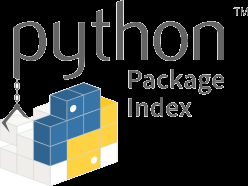
\includegraphics[width=0.4\textwidth,height=0.35\textheight]{pictures/pypi.png}
  \caption{Модулі Python}
\label{function}
  \end{center}
\end{figure}
\end{frame}

\subsection{Модуль random} 
\begin{frame}
\frametitle{Функції модулю random}
\begin{itemize}
  \item<1-> \texttt{random()} - випадкове значення в діапазоні від \texttt{0} до \texttt{1}.
  \item<2-> \texttt{uniform(a, b)} - рівномірно розподілене випадкове значення в діапазоні від \texttt{a} до \texttt{b}. 
  \item<3-> \texttt{randint(a, b)} - ціле випадкове значення в діапазоні від \texttt{a} до \texttt{b}.
  \item<4-> \texttt{randrange(a, b, s)} - випадкове значення в діапазоні від \texttt{a} до \texttt{b} з кроком \texttt{s}.
  \item<5-> \texttt{gauss(mu, sigma)} - нормально розподілене випадкове значення з математичним очікуванням \texttt{mu} та дисперсією \texttt{sigma}.
\end{itemize}

\end{frame}

\begin{frame}
\frametitle{Функції модулю random}
\begin{itemize}
  \item \texttt{choice(lst)} - випадковий елемент списка \texttt{lst}.
  \item \texttt{shuffle(lst)} - випадковим чином перемішує список \texttt{lst}.
  \item \texttt{sample(lst, n)} - повертає список із \texttt{n} випадковим чином обраних унікальних елементів списку \texttt{lst}.
  \item \texttt{seed(n)} - фіксує зерно \texttt{n} генератора випадкових чисел.
\end{itemize}

\end{frame}

\subsection{Зовнішні пакети Python} 
\begin{frame}
\frametitle{Система керування пакетами pip}
\begin{itemize}
  \item NumPy - робота з багатовимірними масивами;
  \item Matplotlib - відображення графіків;
  \item Pygame - реалізація простої 2D-графіки;
  \item Flask - простий веб-фреймворк;
  \item Django - просунутий веб-фреймворк для складних сайтів.
\end{itemize}

Package Installer for Python (pip) — система керування пакетами, що використовується для встановлення і керування пакетами Python. Для встановлення пакету \texttt{some-package-name} виконується команда \texttt{pip install some-package-name}.
\end{frame}

\subsubsection{Пакет Numpy}
\begin{frame}
\frametitle{NumPy: масиви}
NumPy це модуль для Python, який надає загальні математичні та числові операції у вигляді пре-компільованих, швидких функцій. Вони забезпечують функціонал, який можна порівняти із функціоналом MatLab.
\begin{figure}
  \begin{center}
    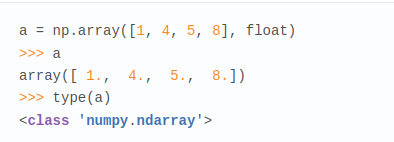
\includegraphics[width=0.5\textwidth,height=0.35\textheight]{pictures/array.png}
  \caption{Об'єкт array}
\label{function}
  \end{center}
\end{figure}
\end{frame}

\begin{frame}
\frametitle{NumPy: методи масивів}
\begin{itemize}
  \item Метод \texttt{a.shape} повертає кількість рядків та стовпців в матриці \texttt{a}.
  \item Метод \texttt{a.dtype} повертає тип змінних, що зберігаються в масиві \texttt{a}.
  \item Метод \texttt{a.fill(n)} заповнює масив \texttt{a} значенням \texttt{n}.
  \item Метод \texttt{a.reshape((n,m))} перетворює масив \texttt{a} у масив розміром \texttt{(n,m)}.
  \item Функція \texttt{np.concatenate(a,b,[c, axis=n])} поєднує матриці \texttt{a} та \texttt{b} (та можливо інші) за розмірністю \texttt{n}.
\end{itemize}

\end{frame}

\begin{frame}
\frametitle{NumPy: методи масивів}
\begin{itemize}
  \item Функція \texttt{np.zeros(s)} (\texttt{np.ones(s)}) створіює матрицю із нулів (одиниць), розмірність задається кортежем \texttt{s}.
  \item Функція \texttt{np.eye(n, k=m)} створіює квадратну матрицю розмірністю \texttt{n} із одиницями по   \texttt{m}-ій діагоналі.
  \item Стандратні операції +, -, *, /, \%, **, математичні функції \texttt{abs}, \texttt{sign}, \texttt{sqrt}, \texttt{log}, \texttt{log10}, \texttt{exp}, тригонометричні функції та оператори \texttt{floor},  \texttt{ceil}  застосовуються до масивів поелементно.
  \item Включено важливі математичні константи \texttt{np.pi} та \texttt{np.e}.

\end{itemize}

\end{frame}

\subsubsection{Пакет SciPy}
\begin{frame}
\frametitle{Можливості SciPy}
\begin{table}
  \caption{Модулі SciPy}
  \label{tab:}

  \begin{center}
    \begin{tabular}{|c|c|}
    \hline
      \textbf{Модуль} & \textbf{Використання} \\
      \hline
      scipy.constants & Математичні та фізичні константи\\
      \hline
      scipy.special & Спеціальні функції математичної фізики\\
      \hline
      scipy.integrate & Чисельне інтегрування\\
      \hline
      scipy.optimize & Максимум/мінімум користувацьких функції\\
      \hline
      scipy.linalg & Функції лінійної алгебри\\
      \hline
    \end{tabular}
  \end{center}
\end{table}
\end{frame}

\begin{frame}
\frametitle{Можливості SciPy}
\begin{table}
  \caption{Модулі SciPy}
  \label{tab:}

  \begin{center}
    \begin{tabular}{|c|c|}
    \hline
      \textbf{Модуль} & \textbf{Використання} \\
      \hline
      scipy.sparse & Робота з розрідженими матрицями\\
      \hline
      scipy.interpolate & Методи та класи для інтерполяції\\
      \hline
      scipy.fftpack & Обробка перетворень Фур'є\\
      \hline
      scipy.signal & Обробка сигналів\\
      \hline
      scipy.stats & Статистичні функції та розподіли\\
      \hline
    \end{tabular}
  \end{center}
\end{table}
\end{frame}

\subsubsection{Пакет Matplotlib}
\begin{frame}
\frametitle{Matplotlib}
Matplotlib - пакет для побудови графіків. Використання:

\texttt{import matplotlib.pyplot as plt}

\begin{figure}
  \begin{center}
    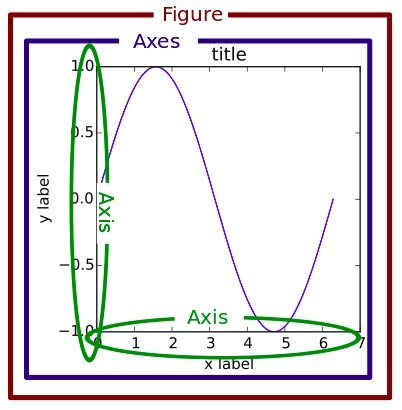
\includegraphics[width=0.5\textwidth,height=0.5\textheight]{pictures/figure-matplotlib.jpg}
  \caption{Ієрархія об'єктів matplotlib}
\label{function}
  \end{center}
\end{figure}
\end{frame}

\begin{frame}
\frametitle{<<Анатомія>> малюнку в Matplotlib}

\begin{figure}
  \begin{center}
    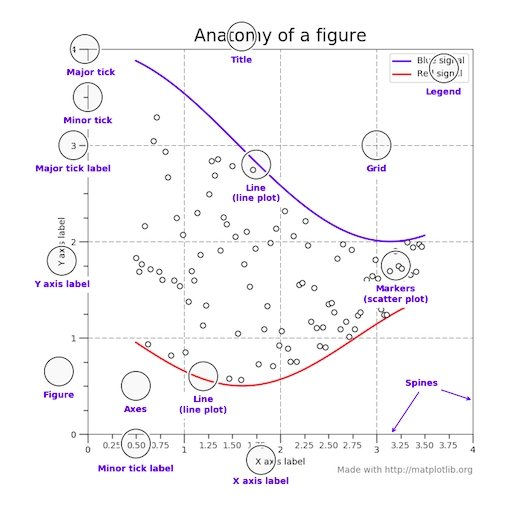
\includegraphics[width=0.6\textwidth,height=0.7\textheight]{pictures/anatomy-matplotlib.jpg}
  \caption{Ієрархія об'єктів matplotlib}
\label{function}
  \end{center}
\end{figure}
\end{frame}

\begin{frame}
\frametitle{Matplotlib: приклад}
\scriptsize
import numpy as np

import matplotlib.pyplot as plt

rng = np.arange(50)

rnd = np.random.randint(0, 10, size=(3, rng.size))

yrs = 1950 + rng

fig, ax = plt.subplots(figsize=(5, 3))

ax.stackplot(yrs, rng + rnd, labels=['Eastasia', 'Eurasia', 'Oceania'])

ax.set\_title('Combined debt growth over time')

ax.legend(loc='upper left')

ax.set\_ylabel('Total debt')

ax.set\_xlim(xmin=yrs[0], xmax=yrs[-1])

fig.tight\_layout()

plt.show()
\normalsize
\end{frame}

\begin{frame}
\frametitle{Matplotlib: приклад}
\begin{itemize}
  \item Після створення трьох часових стовпців (рядів) визначено фігуру (\texttt{fig}), що містить об'єкт \texttt{Axes} (\texttt{plot, ax});
  \item Методи \texttt{ax} викликаються для створення діаграми з розбивкою по областях та додаванням легенди, заголовка та ярлика вісі \texttt{y};
  \item \texttt{tight\_layout()} застосовується до об'єкта Figure для очищення прогалин.
\end{itemize}
\end{frame}

\begin{frame}
\frametitle{Matplotlib: приклад}

\begin{figure}
  \begin{center}
    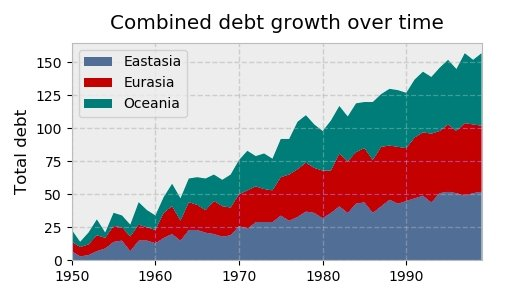
\includegraphics[width=0.6\textwidth,height=0.6\textheight]{pictures/example-matplotlib.jpg}
  \caption{Приклад малюнку в matplotlib}
\label{function}
  \end{center}
\end{figure}
\end{frame}
